\chapter{Introduction}
\label{ch1}

%%%%%%%%%%%%%%%%%%%%%%%%%%%%%%%%%%%%%%%
% IMPORTANT
% THESE LINES MUST APPEAR IN EVERY CHAPTER
% COPY THEM IN ANY NEW CHAPTER
\begin{spacing}{1} 
\ifthenelse{\boolean{mini_list_of_tables}}{
    \minitoc 
}{}
\end{spacing}
\doublespacing 
%%%%%%%%%%%%%%%%%%%%%%%%%%%%%%%%%%%%%%%


\section{Title section}

Let's cite! The Einstein's journal paper \cite{einstein} and the Dirac's 
book \cite{dirac} are physics related items. 

And some acronyms: \ac{USA} and \ac{LTI} systems.

\begin{figure}
\centering
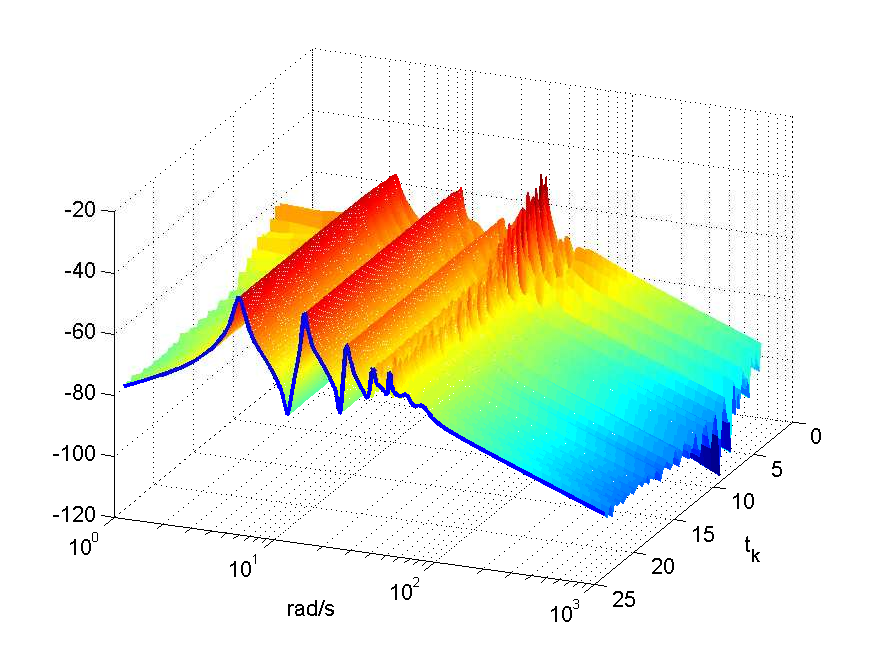
\includegraphics[width=0.8\columnwidth]{imgs/buildmagnitude.pdf}
\caption[Short description for list of figures]{This figure is taken from \cite{Sca:16}.}
\label{fig-magnitude}
\end{figure}%

\subsection{Title subsection}

\kant[1-6]
